\chapter{NHẬN DẠNG CÁC VẬT THỂ DI ĐỘNG}

\chaptermark{Nhận dạng các vật thể di động}
	
\section{CNN}

\section{YOLO - You Only Look Once}

\section{SSD - Single Shot Detector}

\subsection{Giới thiệu về SSD}

  SSD là mô hình single shot detector sử dụng mạng VGG16 để rút trích đặc trưng.Tại mỗi vị trí trên feature map, SSD đặt các default bounding boxes với kích thước, tí lệ khác nhau. Trong quá trình xử lí, SSD sẽ đánh giá và tìm đối tượng trên các bounding box này nhằm tìm ra box phù hợp nhất với đối tượng cần tìm kiếm. Thêm vào đó, bằng việc tìm kiếm trên các feature map khác nhau, SSD có thể tìm kiếm các đối tượng với kích thước khác nhau mà không cần thay đổi kích thước của các bounding box. Thực nghiệm cho thấy, SSD đạt 74.3\% mAP trên tập test của VOC2007, đạt 59 FPS khi sử dụng Nvidia Titan X với kích thước ảnh đầu vào 512 x 512, nhanh hơn Faster R-CNN.
  \\Ý tưởng chính của SSD đến từ việc sử dụng các bounding box, bằng việc khởi tạo sẵn các box tại mỗi vị trí trên ảnh, SSD sẽ tính toán và đánh giá thông tin tại mỗi vị trí xem vị trí đó có vật thể hay không, nếu có thì là vật thể nào, và dựa trên kết quả của các vị trí gần nhau, SSD sẽ tính toán được một box phú hợp nhất bao trọn vật thể.
  \begin{center}
  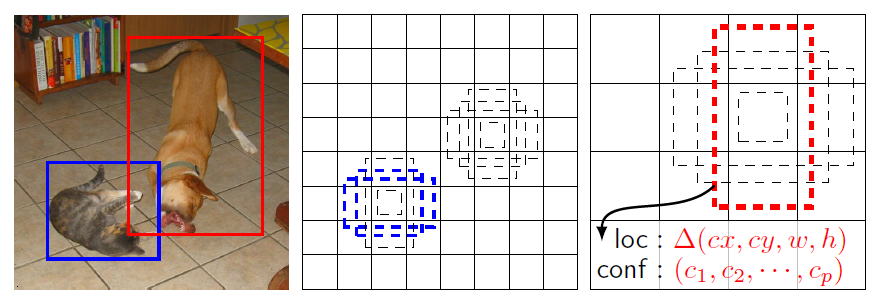
\includegraphics[scale=.5]{ch2/SSD1}
  \end{center}
  Ngoài ra, bằng việc tính toán bounding box trên các feature map khác nhau, tại mỗi tầng feature map, một box sẽ ôm trọn một phần hình ảnh với các kích thước khác nhau. Như trên ví dụ trên, con mèo và con chó có thể được phát hiện ở 2 tầng feature map khác nhau, 2 kích thước và tỉ lệ khác nhau. Thay vì sử dụng 1 box và thay đổi kích thước box cho phù hợp với vật thể, thì SSD dử dụng nhiều box trên nhiều tầng, từ đó tổng hợp ra vị trí và kích thước box kết quả. Bằng việc loại trừ các region proposal, SDD có thể đạt được tốc tộ xử lí cao hơn Faster R-CNN
  \subsubsection{Kiến trúc của SSD}
  \begin{center}
  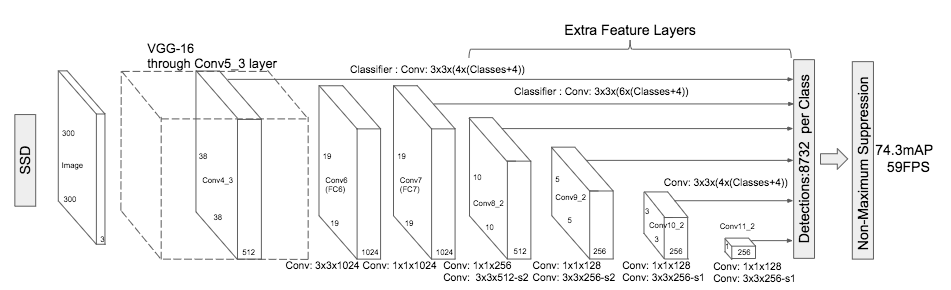
\includegraphics[scale=.5]{ch2/SSD2}
  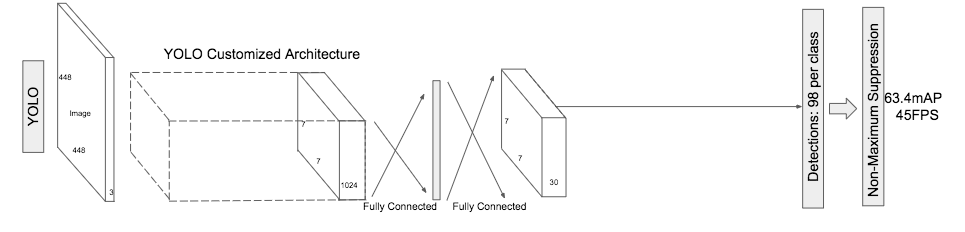
\includegraphics[scale=.5]{ch2/SSD3}
  \end{center}
  Kiến trúc của SSD được xây dựng trên VGG-16 được loại bỏ tầng fully-connected. Lí do mà VGG-16 được sử dụng như tầng cơ sở là vì sự hiệu quả của nó trong bài toán phân loại ảnh với các ảnh có độ phân giải cao. Thay vì sử dụng tầng fully-connected của VGG như của YOLO, một tập các tầng convolution phụ trợ được thêm vào, vì vậy ta có thể trích xuất được các features với nhiều tỉ lệ khác nhau, và giảm gần kích thước của đầu vào trong từng tầng mạng.
  \paragraph{Default boxes}
  \mbox{}\\Trên một feature map kích cỡ \( m \times n\), tại mỗi vị trí cell hay tại mỗi pixel, khởi tạo các default bounding box, các box này có vai trò giống như các anchor của Faster R-CNN. Tuy nhiên, vì vị trí mỗi cell cố định nên các box này cũng sẽ được cố định. Tại mỗi cell, giả sử khởi tạo kk box, SSD tính toán phân loại cc class và đồng thời tính toán xem hình dáng của box như thế nào như toạ độ \((cx,cy)\), dài và rộng \((w,h)\) Vậy tổng số tính toán là \((c+4) k \times m \times n \)

\subsection{Training}
  Việc training SSD yêu cầu cung cấp thông tin về các groundtruth của vật thể bao gồm các thông tin về class, shape.
  \paragraph{Tìm các box phù hợp}
  \mbox{}\\Trong quá trình training, ta tiến hành tìm các default box trên các feature map phù hợp với groundtruth bằng cách tìm các box có Intersection over Union (IoU) cao. Công thức tính IoU dựa trên tỉ lệ giữa diện tích vùng trùng nhau giữa 2 tập và diện tích của cả 2 tập hợp lại
  \begin{center}
  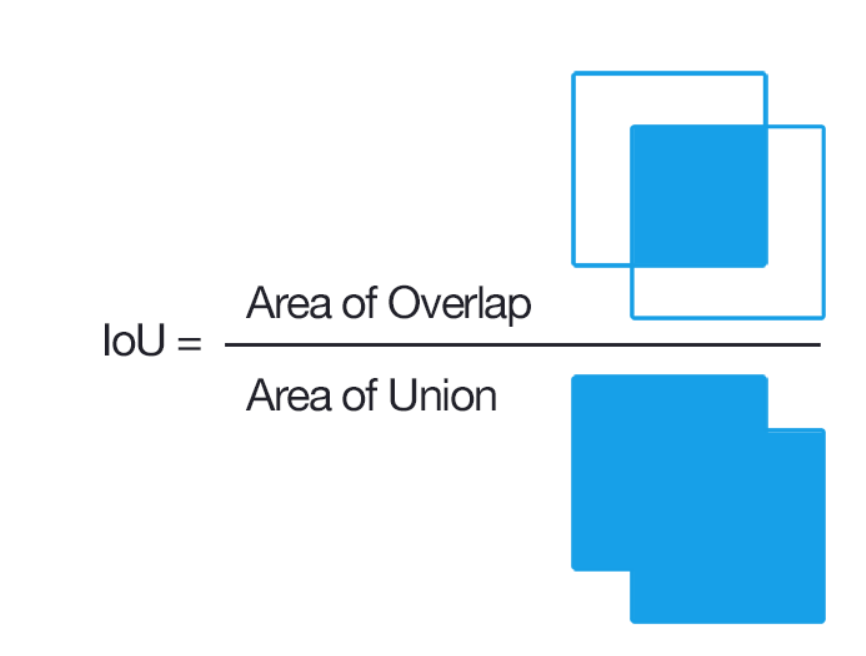
\includegraphics[scale=.5]{ch2/iou}
  \end{center}
  Các box được lọc có chỉ số IoU lớn hơn mức threshol 0.5
  \paragraph{Loss function}
  \mbox{}\\Hàm loss của SSD được xây dựng bằng localization loss để đánh giá việc phát hiện và confidence loss để đánh giá việc phân lớp đối tượng.
  \\Đặt \(x_{ij}^p\) = [1,0] ứng với default box thứ \(i\) khớp với groundtruth thứ \(j\) thuộc lớp \(p\), ta có hàm Loss sau:
  \[L\left( x,c,l,g \right) = \frac{1}{N} \left( L_{conf} \left( x,c \right) + \alpha L_{loc}\left(x,l,g\right)\right)\]
  N ở đây là số lượng những default box phù hợp được tìm ở bước trên. Nếu N = 0 thì Loss = 0. Hàm Loss \(L_{loc}\) được tính bằng Smooth L1 loss giữa box dự đoán \(l\) và groundtruth box \(g\). Với các tham số như điểm chính giữa \(\left(cx,cy\right)\) của default box \(d\) và chiều dài \(w\), chiều rộng \(h\). \(\alpha\) được đặt là 1.
  \paragraph{Localization Loss}
  \mbox{}\[L_{loc}\left( x,l,g \right) = \sum^N_{i\in Pos} \sum_{m\in\{cx,cy,w,h\}} x_{ij}^k smooth_{L1}\left( l_i^m - \hat{g}^m_j\right)\]
  Với:
  \[smooth_{L1} \colon= piewise( abs( x ) < 1, 0.5x^2, abs( x ) - 0.5)\]
  Và:
  \[\hat{g}_j^{cx} = \left( g_j^{cx} - d_j^{cx} \right)/ d_j^w\]
  \[\hat{g}_j^{cy} = \left( g_j^{cy} - d_j^{cy} \right) / d_j^h\]
  \[\hat{g}_j^w = \log\left( \frac{g_j^w}{d_j^w} \right)\]
  \[\hat{g}_j^h = \log\left( \frac{g_j^h}{d^h_i} \right)\]
  \paragraph{Confidence Loss}
  \mbox{}\[L_{conf} \left( x,c \right) = - \sum_{i \in Pos}^N x_{ij}^p \log \left( \hat{c}_i^p \right) - \sum_{i \in N eg} \log\left( \hat{c}_i^p \right)\]
  Với:
  \[\hat{c}_i^p = \frac{\exp\left( c_i^p \right)}{\sum_p \exp\left( c_i^p \right)}\]
  \paragraph{Chọn kích thước và tỉ lệ cho default box}
  \mbox{}\\Các feature map ở độ sâu khác nhau sẽ có kích thước khác nhau, vì vậy, kích thước của các default box cũng được thay đôi theo độ sâu của feature map. Ví dụ với độ sâu là m (bao gồm m feature map tại bước detect):\[s_k = s_{min} + \frac{s_{max} - s_{min}}{m - 1} \left( k - 1 \right), \text{k} \in \left[1,m \right] \text{,} s_{min}=0.2 \text{,} s_{max}=0.9\]
  Vậy với m = 3, ta lần lượt sẽ có \(s_1 = 0.2, s_2 = 0.55, s_3 = 0.9\)
  \\Với tỉ lệ giữa chiều dài và rộng của box, sẽ được tính với \(a_r \in { 1, 2, 3, \frac{1}{2}, \frac{1}{3}}\)
  \\Chiều dài và rộng có thể được tính từ \(a_r\):
  \[w_k^a = s_k \sqrt{a_r}\]
  \[h_k^a = s_k / \sqrt{a_r}\]
  Với trường hợp tỉ lệ bằng 1, ta thêm 1 box nữa với kích thước là \({s\prime}_k = \sqrt{s_ks_k+1}\) Như vậy, trên một vị trí của feature map sẽ có tổng cộgn 6 bounding box. Tâm điểm của mỗi box sẽ được tính bằng:
  \[\left( \frac{i+0.5}{\vert f_k \vert}, \frac{j+0.5}{\vert f_k \vert} \right)\]
  Với \(\vert f_k \vert\) là kích cỡ cửa feature map hình vuông. \(i , j\) là vị trí của cell.

\newpage